\documentclass[11pt,]{article}
\usepackage[]{mathpazo}
\usepackage{amssymb,amsmath}
\usepackage{ifxetex,ifluatex}
\usepackage{fixltx2e} % provides \textsubscript
\ifnum 0\ifxetex 1\fi\ifluatex 1\fi=0 % if pdftex
  \usepackage[T1]{fontenc}
  \usepackage[utf8]{inputenc}
\else % if luatex or xelatex
  \ifxetex
    \usepackage{mathspec}
  \else
    \usepackage{fontspec}
  \fi
  \defaultfontfeatures{Ligatures=TeX,Scale=MatchLowercase}
\fi
% use upquote if available, for straight quotes in verbatim environments
\IfFileExists{upquote.sty}{\usepackage{upquote}}{}
% use microtype if available
\IfFileExists{microtype.sty}{%
\usepackage{microtype}
\UseMicrotypeSet[protrusion]{basicmath} % disable protrusion for tt fonts
}{}
\usepackage[margin=1in]{geometry}
\usepackage{hyperref}
\hypersetup{unicode=true,
            pdftitle={Case Study: Predicting the outcomes of the 2017 Dutch General Elections},
            pdfauthor={Ilse van Beelen, Floor Komen},
            pdfkeywords={put some keywords here},
            pdfborder={0 0 0},
            breaklinks=true}
\urlstyle{same}  % don't use monospace font for urls
\usepackage{natbib}
\bibliographystyle{plainnat}
\usepackage{color}
\usepackage{fancyvrb}
\newcommand{\VerbBar}{|}
\newcommand{\VERB}{\Verb[commandchars=\\\{\}]}
\DefineVerbatimEnvironment{Highlighting}{Verbatim}{commandchars=\\\{\}}
% Add ',fontsize=\small' for more characters per line
\usepackage{framed}
\definecolor{shadecolor}{RGB}{248,248,248}
\newenvironment{Shaded}{\begin{snugshade}}{\end{snugshade}}
\newcommand{\KeywordTok}[1]{\textcolor[rgb]{0.13,0.29,0.53}{\textbf{#1}}}
\newcommand{\DataTypeTok}[1]{\textcolor[rgb]{0.13,0.29,0.53}{#1}}
\newcommand{\DecValTok}[1]{\textcolor[rgb]{0.00,0.00,0.81}{#1}}
\newcommand{\BaseNTok}[1]{\textcolor[rgb]{0.00,0.00,0.81}{#1}}
\newcommand{\FloatTok}[1]{\textcolor[rgb]{0.00,0.00,0.81}{#1}}
\newcommand{\ConstantTok}[1]{\textcolor[rgb]{0.00,0.00,0.00}{#1}}
\newcommand{\CharTok}[1]{\textcolor[rgb]{0.31,0.60,0.02}{#1}}
\newcommand{\SpecialCharTok}[1]{\textcolor[rgb]{0.00,0.00,0.00}{#1}}
\newcommand{\StringTok}[1]{\textcolor[rgb]{0.31,0.60,0.02}{#1}}
\newcommand{\VerbatimStringTok}[1]{\textcolor[rgb]{0.31,0.60,0.02}{#1}}
\newcommand{\SpecialStringTok}[1]{\textcolor[rgb]{0.31,0.60,0.02}{#1}}
\newcommand{\ImportTok}[1]{#1}
\newcommand{\CommentTok}[1]{\textcolor[rgb]{0.56,0.35,0.01}{\textit{#1}}}
\newcommand{\DocumentationTok}[1]{\textcolor[rgb]{0.56,0.35,0.01}{\textbf{\textit{#1}}}}
\newcommand{\AnnotationTok}[1]{\textcolor[rgb]{0.56,0.35,0.01}{\textbf{\textit{#1}}}}
\newcommand{\CommentVarTok}[1]{\textcolor[rgb]{0.56,0.35,0.01}{\textbf{\textit{#1}}}}
\newcommand{\OtherTok}[1]{\textcolor[rgb]{0.56,0.35,0.01}{#1}}
\newcommand{\FunctionTok}[1]{\textcolor[rgb]{0.00,0.00,0.00}{#1}}
\newcommand{\VariableTok}[1]{\textcolor[rgb]{0.00,0.00,0.00}{#1}}
\newcommand{\ControlFlowTok}[1]{\textcolor[rgb]{0.13,0.29,0.53}{\textbf{#1}}}
\newcommand{\OperatorTok}[1]{\textcolor[rgb]{0.81,0.36,0.00}{\textbf{#1}}}
\newcommand{\BuiltInTok}[1]{#1}
\newcommand{\ExtensionTok}[1]{#1}
\newcommand{\PreprocessorTok}[1]{\textcolor[rgb]{0.56,0.35,0.01}{\textit{#1}}}
\newcommand{\AttributeTok}[1]{\textcolor[rgb]{0.77,0.63,0.00}{#1}}
\newcommand{\RegionMarkerTok}[1]{#1}
\newcommand{\InformationTok}[1]{\textcolor[rgb]{0.56,0.35,0.01}{\textbf{\textit{#1}}}}
\newcommand{\WarningTok}[1]{\textcolor[rgb]{0.56,0.35,0.01}{\textbf{\textit{#1}}}}
\newcommand{\AlertTok}[1]{\textcolor[rgb]{0.94,0.16,0.16}{#1}}
\newcommand{\ErrorTok}[1]{\textcolor[rgb]{0.64,0.00,0.00}{\textbf{#1}}}
\newcommand{\NormalTok}[1]{#1}
\usepackage{graphicx,grffile}
\makeatletter
\def\maxwidth{\ifdim\Gin@nat@width>\linewidth\linewidth\else\Gin@nat@width\fi}
\def\maxheight{\ifdim\Gin@nat@height>\textheight\textheight\else\Gin@nat@height\fi}
\makeatother
% Scale images if necessary, so that they will not overflow the page
% margins by default, and it is still possible to overwrite the defaults
% using explicit options in \includegraphics[width, height, ...]{}
\setkeys{Gin}{width=\maxwidth,height=\maxheight,keepaspectratio}
\IfFileExists{parskip.sty}{%
\usepackage{parskip}
}{% else
\setlength{\parindent}{0pt}
\setlength{\parskip}{6pt plus 2pt minus 1pt}
}
\setlength{\emergencystretch}{3em}  % prevent overfull lines
\providecommand{\tightlist}{%
  \setlength{\itemsep}{0pt}\setlength{\parskip}{0pt}}
\setcounter{secnumdepth}{0}
% Redefines (sub)paragraphs to behave more like sections
\ifx\paragraph\undefined\else
\let\oldparagraph\paragraph
\renewcommand{\paragraph}[1]{\oldparagraph{#1}\mbox{}}
\fi
\ifx\subparagraph\undefined\else
\let\oldsubparagraph\subparagraph
\renewcommand{\subparagraph}[1]{\oldsubparagraph{#1}\mbox{}}
\fi

%%% Use protect on footnotes to avoid problems with footnotes in titles
\let\rmarkdownfootnote\footnote%
\def\footnote{\protect\rmarkdownfootnote}

%%% Change title format to be more compact
\usepackage{titling}

% Create subtitle command for use in maketitle
\newcommand{\subtitle}[1]{
  \posttitle{
    \begin{center}\large#1\end{center}
    }
}

\setlength{\droptitle}{-2em}

  \title{Case Study: Predicting the outcomes of the 2017 Dutch General Elections}
    \pretitle{\vspace{\droptitle}\centering\huge}
  \posttitle{\par}
    \author{Ilse van Beelen, Floor Komen}
    \preauthor{\centering\large\emph}
  \postauthor{\par}
      \predate{\centering\large\emph}
  \postdate{\par}
    \date{January 15, 2019}

\usepackage{float}

\begin{document}
\maketitle
\begin{abstract}
Put the abstract over here
\end{abstract}

\section{1. Introduction}\label{introduction}

\subsection{1.1 Motivation}\label{motivation}

For this case study, it was decided to combine the outcome from the
Dutch elections of 2017 and demographic data. Both are collected per
municipality and are well maintained and reliable. This makes A lot of
information is available for both in the Netherlands. This will
hopefully result in observing voting trends per demographic group. The
final goal is to validate the model for making futyre predictions.

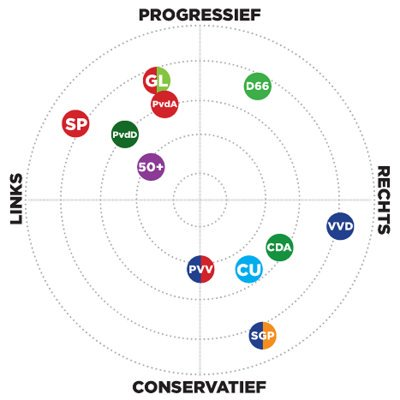
\includegraphics[width=2.60417in]{Partijlandschap.jpg} \textbf{Dutch
political parties}\\
This figure displays the diffences between the political parties in the
Netherlands. The Netherlands has a total of 13 parties. This
investigation focusses on only one party. This party should not be to
extreme left/right/conservative/progressive and should also be one of
the bigger parties. Otherwise, there is not enough data available,
making the results less reliable. Therefore, party CDA is chosen.

In this research the above described demographics are chosen because of
their influence on a municipality level. The expectation is that a
municipality with more non-western residents for example votes different
than a municipality with less non-western residents. This is the same
for the other two demographics. Other demographics are also researched,
for example gender, but on a municipality level there is no large
difference between the amount of men and women per municipality. So that
is a more interesting demographic to research on an individual level.
\emph{The standardized income per municipality} are given in thousands.
\emph{the urban index of a municipality} is a database with five
categories per municipality. These five categories are:

\begin{itemize}
\item Really strong urbanity (more than 2500 addresses per $km^2$) 
\item Strong urbanity (1500-2500 addresses per $km^2$) 
\item Moderate urbanity (1000- 1500 addresses per $km^2$) 
\item Little urbanity (500-1000 addresses per $km^2$)  
\item No urbanity (less than 500 addresses per $km^2$)
\end{itemize}

Per municipality the amount of \(km^2\) per category is given. The
\emph{non-west residents per municipality} is given in an amount per
municipality, also the total amount of residents is given per
municipality.

\subsection{1.2 Data sources}\label{data-sources}

\textbf{Electoral data} For the electoral data, the results of the 2017
general election are used. This is the most recent national election and
is of the most important election type in the Netherlands. Furthermore,
it had a turnup of 81.9\%. Therefore, it seems plausible that the data
for this election is representative of the political makeup of different
municipalities. We downloaded the raw data directly from the official
government source.\footnote{\url{https://data.overheid.nl/data/dataset/verkiezingsuitslag-tweede-kamer-2017}}
This contained a .csv file with the raw number of votes for every party
in every municipality.

\textbf{Demographical data}\\
We got our demographical data from the CBS, the official Dutch
statistical agency.\footnote{\url{https://opendata.cbs.nl/statline/\#/CBS/nl/dataset/70072ned/table?ts=1544803364892}}
From the wealth of demographical information available we picked a
handful of attributes that we suspected (based on prior research and
some gut feeling) to be useful as predictor variables. We landed on five
demographical attributes: education grade, average income, age,
urbanization and the amount of people with a non-western background.
Note that the data we downloaded from the CBS site usually had to be
transformed to get it in a useful predictor variable format. The
specifics of these are described in the next section.

\subsection{1.3 Data cleaning}\label{data-cleaning}

An extensive amount of data cleaning had to be done. Below these steps
are describes and a small part of code is displayed.

\textbf{Electoral data}

\textbf{Demographical data}

The variable \emph{non-western residents} are divided in three groups:

\begin{itemize}
\item Municipalities with less than 5 % non-western residents 
\item Municipalities with 5-10 % non-western resident 
\item Municipalities with mre than 10 % non-western residents
\end{itemize}

\begin{Shaded}
\begin{Highlighting}[]
\NormalTok{Data_CDA}\OperatorTok{$}\NormalTok{Non_west <-}\StringTok{ }\KeywordTok{ifelse}\NormalTok{(Data_CDA}\OperatorTok{$}\NormalTok{Non_west_frac }\OperatorTok{<}\StringTok{ }\FloatTok{0.05}\NormalTok{, }\DecValTok{1}\NormalTok{, }\OtherTok{NA}\NormalTok{)}
\NormalTok{Data_CDA}\OperatorTok{$}\NormalTok{Non_west <-}\StringTok{ }\KeywordTok{ifelse}\NormalTok{(Data_CDA}\OperatorTok{$}\NormalTok{Non_west_frac }\OperatorTok{>=}\StringTok{ }\FloatTok{0.05} \OperatorTok{&}\StringTok{ }\NormalTok{Data_CDA}\OperatorTok{$}\NormalTok{Non_west_frac }\OperatorTok{<}\StringTok{ }
\StringTok{    }\FloatTok{0.1}\NormalTok{, }\DecValTok{2}\NormalTok{, Data_CDA}\OperatorTok{$}\NormalTok{Non_west)}
\NormalTok{Data_CDA}\OperatorTok{$}\NormalTok{Non_west <-}\StringTok{ }\KeywordTok{ifelse}\NormalTok{(Data_CDA}\OperatorTok{$}\NormalTok{Non_west_frac }\OperatorTok{>=}\StringTok{ }\FloatTok{0.1}\NormalTok{, }\DecValTok{3}\NormalTok{, Data_CDA}\OperatorTok{$}\NormalTok{Non_west)}
\NormalTok{Data_CDA}\OperatorTok{$}\NormalTok{Non_west <-}\StringTok{ }\KeywordTok{as.factor}\NormalTok{(Data_CDA}\OperatorTok{$}\NormalTok{Non_west)}
\end{Highlighting}
\end{Shaded}

At last, the electoral data and demographic data are combined again.
Only the municipality Boxmeer is removed, due to a mistake not all the
votes are reported here\footnote{\url{https://www.gelderlander.nl/boxmeer/7-600-stemmen-in-boxmeer-niet-meegenomen-in-uitslag-verkiezingen~a063ee9e/}}.
The final dataset has no NAs

\begin{Shaded}
\begin{Highlighting}[]
\KeywordTok{summary}\NormalTok{(Data_CDA)}
\end{Highlighting}
\end{Shaded}

\begin{verbatim}
##      Muni              CDA_frac       Urban_index     High_educated_frac
##  Length:366         Min.   :0.0310   Min.   :0.0000   Min.   :0.1200    
##  Class :character   1st Qu.:0.1170   1st Qu.:0.6623   1st Qu.:0.2200    
##  Mode  :character   Median :0.1420   Median :1.2305   Median :0.2600    
##                     Mean   :0.1528   Mean   :1.4280   Mean   :0.2662    
##                     3rd Qu.:0.1820   3rd Qu.:2.1750   3rd Qu.:0.3000    
##                     Max.   :0.4200   Max.   :3.7890   Max.   :0.4700    
##   Mean_income    Non_west_frac        CDA_abs        Total_abs     
##  Min.   :20.80   Min.   :0.01000   Min.   :  421   Min.   :  2727  
##  1st Qu.:24.30   1st Qu.:0.03000   1st Qu.: 1737   1st Qu.: 11516  
##  Median :25.60   Median :0.05000   Median : 2510   Median : 16915  
##  Mean   :25.91   Mean   :0.06574   Mean   : 3254   Mean   : 25162  
##  3rd Qu.:27.00   3rd Qu.:0.08000   3rd Qu.: 4023   3rd Qu.: 27087  
##  Max.   :41.80   Max.   :0.38000   Max.   :18813   Max.   :440854  
##   Frac_60plus     Non_west
##  Min.   :0.0700   1:178   
##  1st Qu.:0.1200   2:111   
##  Median :0.1300   3: 77   
##  Mean   :0.1327           
##  3rd Qu.:0.1400           
##  Max.   :0.1800
\end{verbatim}

\subsection{1.3 Data visualisation}\label{data-visualisation}

In this part the cleaned data is visualized, so that a good picture can
be obtained of the current data. First of all some demographics of data
will be showed. In figure \ref{1} of the \emph{parties}, \emph{the urban
index}, \emph{the percentage of highly educated residents}, \emph{the
mean income}, \emph{The non west residents factor} and * the percentage
60 plus* are plotted. As you can see in the plot, they are normal
distributed. Because of the low values at the x-axis, the CDA,
GroenLinks, 60 plus percentage and the highly educated densities are
above 1. The area beneath the curve sums to 1, so it is correct.

\begin{figure}[H]

{\centering 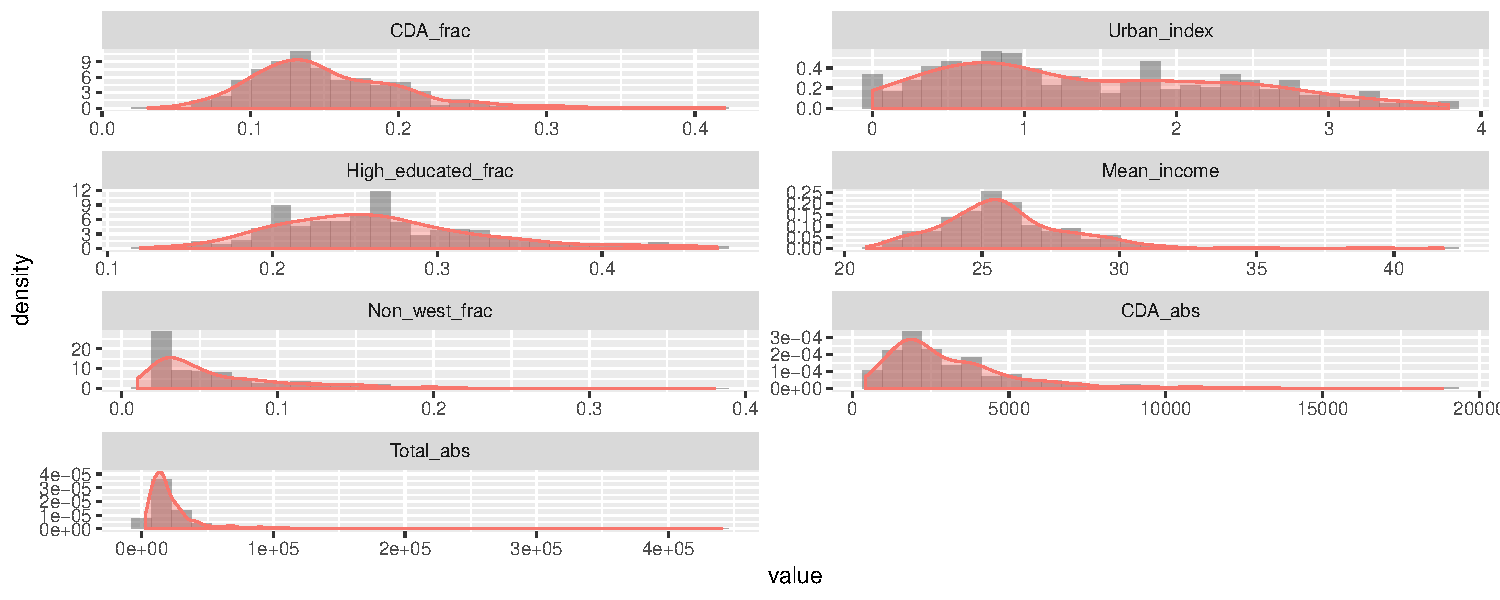
\includegraphics{Report_files/figure-latex/demographics_data-1} 

}

\caption{\label{1} Density plot}\label{fig:demographics_data}
\end{figure}

\textbf{Correlation heatmap} In this heatmap (figure \ref{2}) the
correlation between explanatory and respons variable are showed. The red
color means a positive relation, the purple color means a negative
relation. The non\_west variable is not taken into account, because it
is a factor and the other variables are continous.

\begin{figure}[H]

{\centering 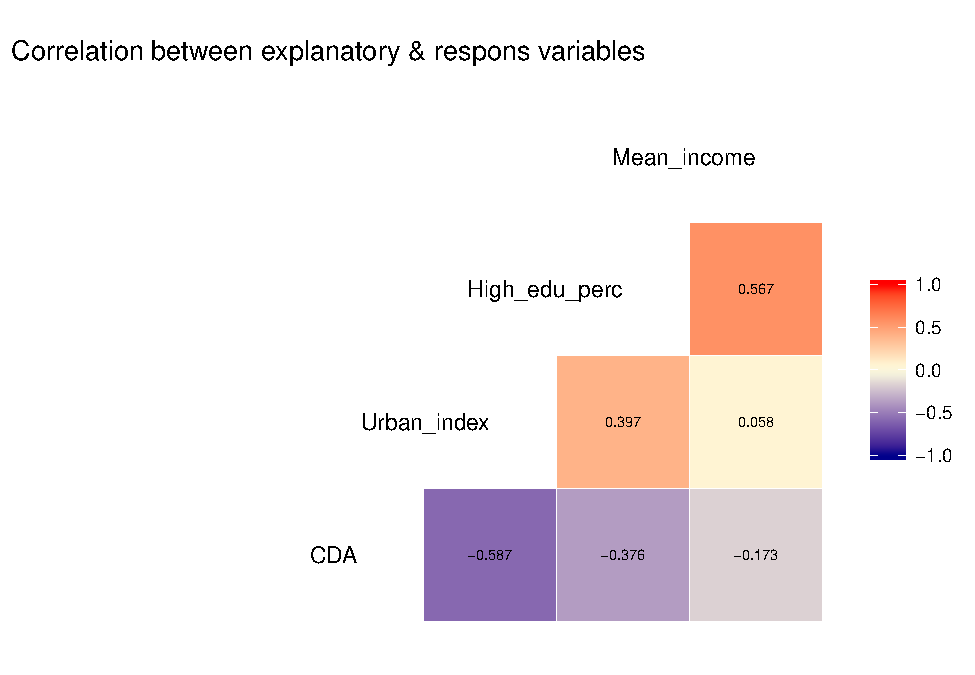
\includegraphics{Report_files/figure-latex/correlation_heatmap-1} 

}

\caption{\label{2}Correlation between explanatory and respons variables}\label{fig:correlation_heatmap}
\end{figure}

\textbf{Multilineair plots CDA } In these two plots you can see a
scatterplot with on the y-axis the votes for CDA in percentages and on
the x-axis on the left graph the mean income per municipality in 1000
euro. The right plot has the urbanity index as x-axis. As you can see,
the trend is that when the mean income goes up, the votes for CDA goes
down. Same with the urbanity index. In the model formulation graph these
trends are checked.

\begin{figure}[H]

{\centering 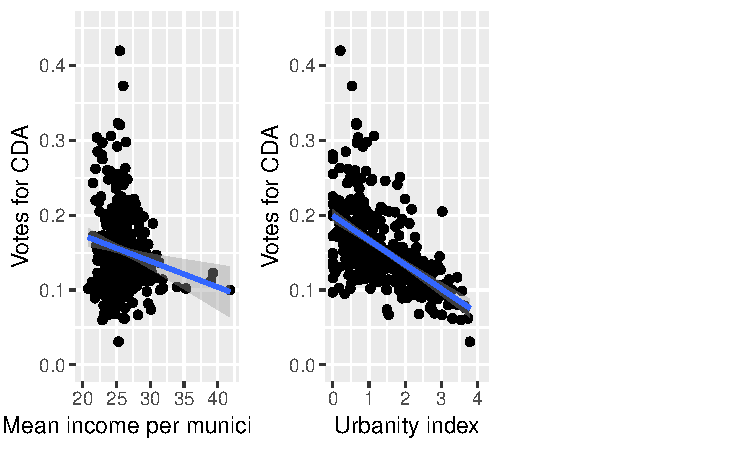
\includegraphics{Report_files/figure-latex/unnamed-chunk-6-1} 

}

\caption{\label{3}Scatterplots CDA}\label{fig:unnamed-chunk-6}
\end{figure}

\textbf{Multilinear plots explanatory variables} These three plots are
scatterplots about explanatory variables.

\begin{figure}[H]

{\centering 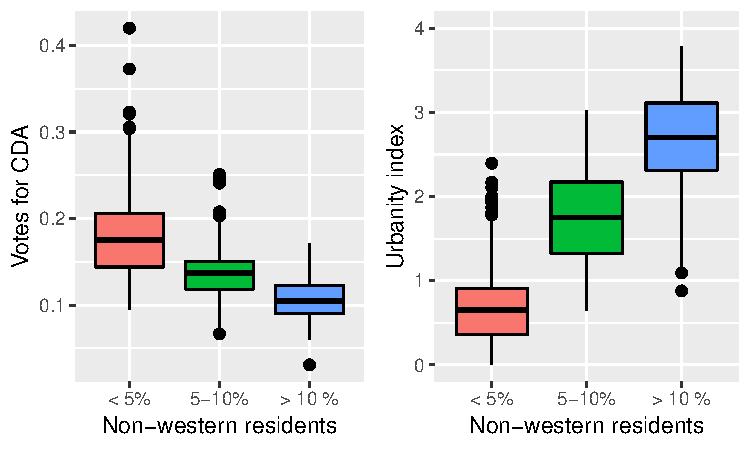
\includegraphics{Report_files/figure-latex/unnamed-chunk-7-1} 

}

\caption{\label{5}Scatterplot explanatory variables}\label{fig:unnamed-chunk-71}
\end{figure}\begin{figure}[H]

{\centering 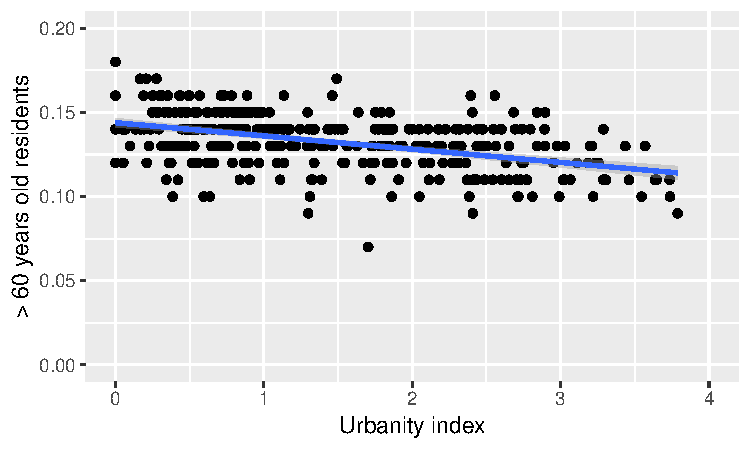
\includegraphics{Report_files/figure-latex/unnamed-chunk-7-2} 

}

\caption{\label{5}Scatterplot explanatory variables}\label{fig:unnamed-chunk-72}
\end{figure}

\textbf{Multiple boxplots} In this graph boxplots are made, to compare
some variables. A boxplot is a standardized way to display the
distribution of data. It gives the minimum, first quartile, median,
third quartile and the maximum. If there are any outliers, the boxplot
is extended with those. The line within the box is the median, the first
and third quartile are the down- and upside of the box. The length of
the box is the Inter Quartile Range (IQR). The minimum and maximum are
1.5XIQR distance. Outliers are thus further away than 1.5XIQR.

\begin{figure}[H]

{\centering 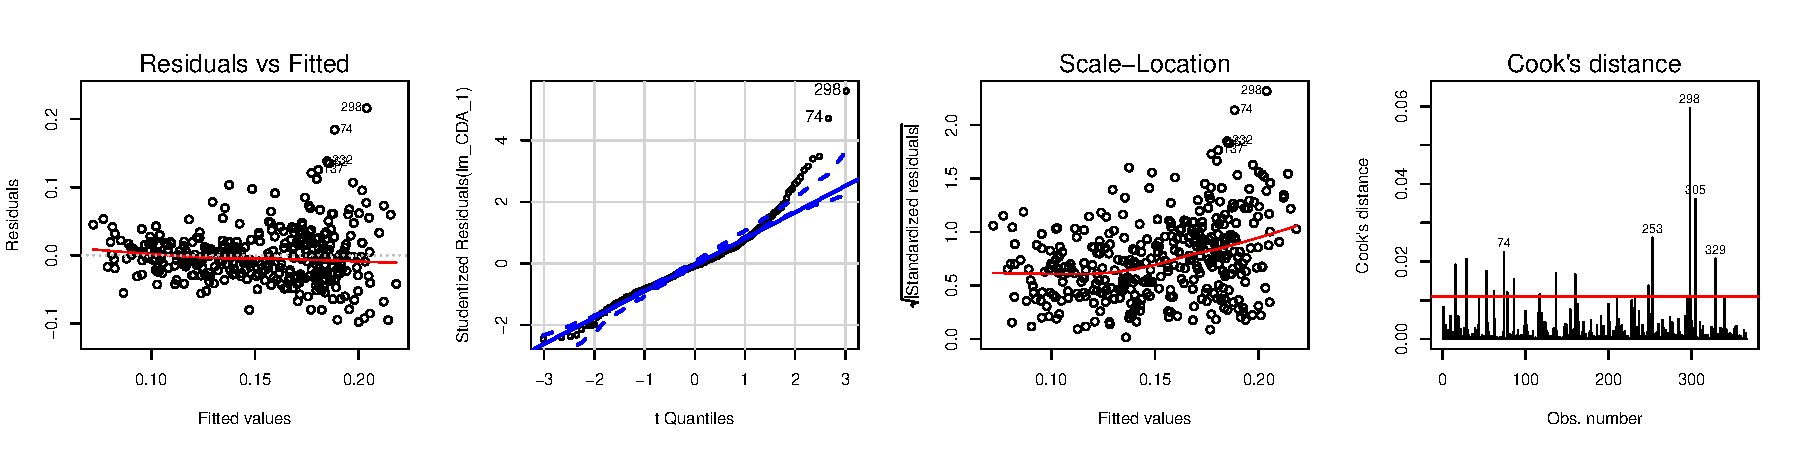
\includegraphics{Report_files/figure-latex/unnamed-chunk-8-1} 

}

\caption{\label{6}Three boxplots: Votes for CDA, Votes for GroenLinks and Urbanity index}\label{fig:unnamed-chunk-8}
\end{figure}

\section{2. Multiple linear
regression}\label{multiple-linear-regression}

\subsection{First model}\label{first-model}

\subsection{Final model}\label{final-model}

\subsection{Cross validation}\label{cross-validation}

\section{3. Logistic regression}\label{logistic-regression}

The raw respons variable is the absolute amount of residents per
municipality that voted for CDA. For linear regresssion, we transformed
this variable to a fraction. However, we also know the total amount of
votes per municipality. Therefore, a better fit to our data would be a
binomial model. We use the logit as link function to transform the range
of the respons. The choice for the logit was easily made. Because the
inverse of the logit is directly interpretable as the log-odds ratio.
This link displays the underlaying pattern of our data best. Below, the
formula for our link function:

\(\eta = log(\frac{\theta}{1 - \theta})\)

Where \(\theta\) is the absolute amount of votes for CDA.

In GLM, we still have to make diagnostics plots to visualise if any of
the assumptions for the error-term are violated. The assumptions made
for the error-term in a binomial model are slightly different than for
the linear model. Below we state the assumptions:

\begin{itemize}
\item[] Check deviance residuals
\item[] Leverages are no longer just a function of X and now depend on the response through the weights W.
\end{itemize}

\subsection{First model}\label{first-model-1}

\subsection{Second model}\label{second-model}

\subsection{Final model}\label{final-model-1}

\subsection{Cross validation}\label{cross-validation-1}

\section{4. Discussion}\label{discussion}

\subsection{Limitations}\label{limitations}


\end{document}
